\documentclass[aspectratio=169,11pt]{beamer}

\usepackage[T1]{fontenc}
\usepackage{lmodern}
\usepackage{booktabs}
\usepackage{tikz}
\usepackage{graphicx}
\usepackage{xcolor}
\usepackage{array}
\usepackage{ragged2e}
\usetikzlibrary{arrows.meta,positioning,fit,calc}

\definecolor{ink}{HTML}{132238}
\definecolor{steel}{HTML}{35516B}
\definecolor{teal}{HTML}{007C83}
\definecolor{orange}{HTML}{E07A36}
\definecolor{mist}{HTML}{F3F6F8}
\definecolor{line}{HTML}{D9E2E8}

\usetheme{default}
\setbeamertemplate{navigation symbols}{}
\setbeamertemplate{footline}{\hfill\color{steel}\scriptsize\insertframenumber\, / 4\hspace{0.45cm}\vspace{0.18cm}}
\setbeamertemplate{frametitle}{\vspace{0.25cm}\color{ink}\insertframetitle\par\vspace{0.08cm}\color{teal}\rule{\textwidth}{1.2pt}}
\setbeamercolor{normal text}{fg=ink,bg=white}
\setbeamercolor{structure}{fg=teal}
\setbeamersize{text margin left=0.55cm,text margin right=0.55cm}
\setlength{\parskip}{0.18em}
\renewcommand{\arraystretch}{1.22}

\newcommand{\tagline}[1]{\textcolor{orange}{\small\bfseries #1}}
\newcommand{\metric}[2]{\begin{tikzpicture}\node[fill=mist,rounded corners=2pt,inner sep=7pt,minimum width=2.7cm,minimum height=0.9cm,align=center]{\textcolor{teal}{\Large\bfseries #1}\\[-1pt]\scriptsize #2};\end{tikzpicture}}

\title{Automated SEM Defect Detection}
\subtitle{YOLOS-tiny fine-tuning with imbalance-aware sampling}
\author{Semiconductor Inspection Study}
\date{\today}

\begin{document}

% PAGE 1
\begin{frame}[plain]
  \begin{tikzpicture}[remember picture,overlay]
    \fill[ink] (current page.north west) rectangle (current page.south east);
    \fill[teal] (current page.north east) -- ([xshift=-4.2cm]current page.north east) -- ([xshift=-1.4cm,yshift=-\paperheight]current page.north east) -- (current page.south east) -- cycle;
    \draw[orange,line width=4pt] ([xshift=0.7cm,yshift=-1.15cm]current page.north west) -- ([xshift=5.1cm,yshift=-1.15cm]current page.north west);
  \end{tikzpicture}
  \vspace{0.6cm}
  {\tagline{VISION-BASED PROCESS MONITORING}}\\[0.35cm]
  {\color{white}\fontsize{29}{34}\selectfont\bfseries Automated\\SEM Defect Detection}\par
  \vspace{0.35cm}
  {\color{white!78}\large YOLOS-tiny fine-tuning for bridge, gap, and line-collapse defects}\par
  \vfill
  \begin{columns}[T]
    \column{0.62\textwidth}
    {\color{white!88}\normalsize A compact object-detection pipeline for semiconductor image review, designed to turn annotated microscopy data into localized, auditable defect candidates.}
    \column{0.32\textwidth}
    \raggedleft{\color{white}\small\bfseries Project brief\\[2pt]\color{white!70}COCO data\\YOLOS detector\\Weighted sampling}
  \end{columns}
\end{frame}

% PAGE 2
\begin{frame}{1. Dataset and inspection resources}
  \begin{columns}[T]
    \column{0.48\textwidth}
    \tagline{DATA SOURCE}\par\vspace{0.05cm}
    Roboflow COCO export from the \texttt{annotate\_image} dataset. Each image is paired with bounding-box annotations in \texttt{\_annotations.coco.json}. Images are RGB and exported at \textbf{224$\times$224 pixels}.
    \vspace{0.22cm}
    \begin{tabular}{>{\bfseries}p{2.0cm}r r}
      \toprule
      Split & Images & Boxes\\
      \midrule
      Train & 102 & 129\\
      Validation & 9 & 11\\
      \midrule
      Total & 111 & 140\\
      \bottomrule
    \end{tabular}
    \vspace{0.18cm}

    \scriptsize\textcolor{steel}{Class box counts across both splits: bridge 80; gap 31; line\_collapse 29.}

    \column{0.48\textwidth}
    \tagline{WHAT THE LABELS MEAN}\par\vspace{0.05cm}
    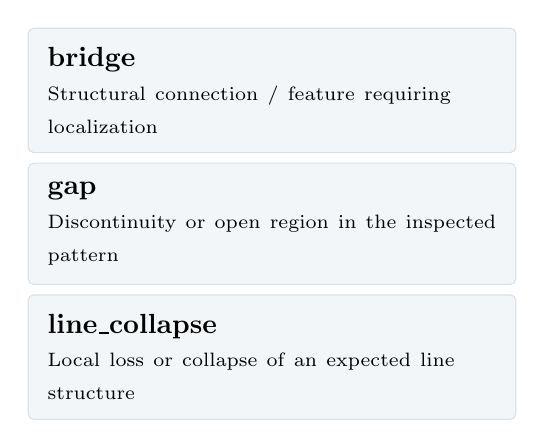
\begin{tikzpicture}[node distance=0.12cm]
      \node[fill=mist,draw=line,rounded corners=2pt,text width=5.7cm,inner sep=7pt] (b) {\textbf{bridge}\\\scriptsize Structural connection / feature requiring localization};
      \node[fill=mist,draw=line,rounded corners=2pt,text width=5.7cm,inner sep=7pt,below=of b] (g) {\textbf{gap}\\\scriptsize Discontinuity or open region in the inspected pattern};
      \node[fill=mist,draw=line,rounded corners=2pt,text width=5.7cm,inner sep=7pt,below=of g] (l) {\textbf{line\_collapse}\\\scriptsize Local loss or collapse of an expected line structure};
    \end{tikzpicture}
    \vspace{0.18cm}
    \tagline{RESOURCES}\par
    \scriptsize COCO annotations \textbullet\ PIL / PyTorch loader \textbullet\ YOLOS image processor \textbullet\ saved checkpoints \textbullet\ prediction visualizations
  \end{columns}
\end{frame}

% PAGE 3
\begin{frame}{2. Model, architecture, and proposed fine-tuning}
  \begin{columns}[T]
    \column{0.42\textwidth}
    \tagline{MODEL}\par\vspace{0.05cm}
    \textbf{YOLOS-tiny} (\texttt{hustvl/yolos-tiny}) is a Vision Transformer detector. It treats detection as set prediction: a fixed collection of detection queries is matched to ground-truth objects with Hungarian matching.
    \vspace{0.16cm}
    \begin{itemize}\setlength\itemsep{1pt}\small
      \item Patch-based image tokenization
      \item Transformer self-attention for global context
      \item Detection tokens produce class and box predictions
      \item Pretrained head replaced for 3 project classes
    \end{itemize}
    \vspace{0.1cm}
    \tagline{TRAINING CONTROL}\par
    \scriptsize 80-epoch maximum \textbullet\ batch size 2 \textbullet\ learning rate $5\times10^{-5}$ \textbullet\ cosine schedule \textbullet\ validation every epoch \textbullet\ early stopping patience 10

    \column{0.55\textwidth}
    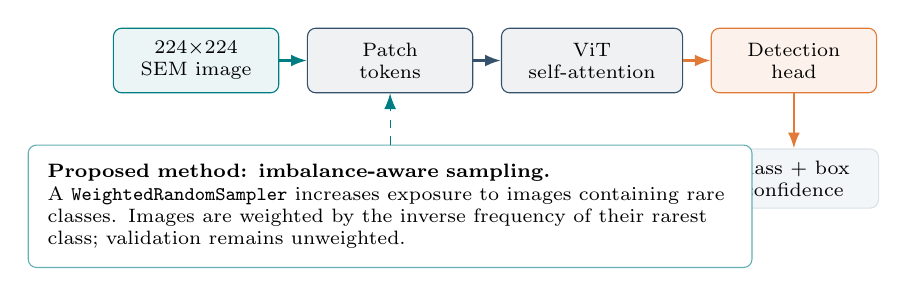
\begin{tikzpicture}[font=\scriptsize, node distance=0.35cm]
      \node[draw=teal,fill=teal!8,rounded corners=3pt,minimum width=2.1cm,minimum height=0.82cm,align=center] (img) {224$\times$224\\SEM image};
      \node[draw=steel,fill=steel!8,rounded corners=3pt,minimum width=2.1cm,minimum height=0.82cm,align=center,right=of img] (patch) {Patch\\tokens};
      \node[draw=steel,fill=steel!8,rounded corners=3pt,minimum width=2.3cm,minimum height=0.82cm,align=center,right=of patch] (vit) {ViT\\self-attention};
      \node[draw=orange,fill=orange!10,rounded corners=3pt,minimum width=2.1cm,minimum height=0.82cm,align=center,right=of vit] (head) {Detection\\head};
      \draw[-{Latex[length=2mm]},thick,teal] (img) -- (patch);
      \draw[-{Latex[length=2mm]},thick,steel] (patch) -- (vit);
      \draw[-{Latex[length=2mm]},thick,orange] (vit) -- (head);
      \node[draw=line,fill=mist,rounded corners=3pt,minimum width=2.15cm,minimum height=0.75cm,align=center,below=0.7cm of head] (out) {class + box\\confidence};
      \draw[-{Latex[length=2mm]},thick,orange] (head) -- (out);
      \node[draw=teal!60,fill=white,rounded corners=3pt,text width=8.7cm,inner sep=7pt,below=0.65cm of patch] (method) {\textbf{Proposed method: imbalance-aware sampling.}\\\scriptsize A \texttt{WeightedRandomSampler} increases exposure to images containing rare classes. Images are weighted by the inverse frequency of their rarest class; validation remains unweighted.};
      \draw[-{Latex[length=2mm]},dashed,teal] (method.north) -- (patch.south);
    \end{tikzpicture}
  \end{columns}
\end{frame}

% PAGE 4
\begin{frame}{3. Inference, benchmark context, and next steps}
  \begin{columns}[T]
    \column{0.36\textwidth}
    \tagline{QUALITATIVE INFERENCE}\par\vspace{0.05cm}
    \includegraphics[width=0.9\linewidth]{prediction\_fig26\_jpg.rf.089135d86dd47e4685a2e9eeba514619.jpg}
    \vspace{0.03cm}
    {\scriptsize\textcolor{steel}{Weighted-model visualization on a validation image. Red boxes indicate predictions above the inference threshold used by \texttt{infer\_yolos.py}.}}
    \column{0.60\textwidth}
    \tagline{READING THE CURRENT RESULT}\par
    \small The pipeline is operational and produces localized candidates, but the available prediction file contains many low-confidence detections. The 9-image validation set is too small for a stable performance claim.
    \vspace{0.12cm}
    \begin{tabular}{p{2.2cm}p{2.45cm}p{2.45cm}}
      \toprule
      \textbf{Comparison} & \textbf{Current evidence} & \textbf{Interpretation}\\
      \midrule
      Standard YOLOS & Unweighted checkpoint available & Baseline for controlled ablation\\
      Weighted YOLOS & Rare-class sampling + visualization & Better exposure, not guaranteed better AP\\
      Industry SOTA & No matched benchmark in this run & Must be measured on the same split\\
      \bottomrule
    \end{tabular}
    \vspace{0.12cm}
    \tagline{WHY VALUES MAY BE LOW}\par
    \scriptsize\begin{itemize}\setlength\itemsep{0pt}\item Dataset is very small and class-imbalanced.\item 224$\times$224 resizing can erase fine semiconductor features.\item Only 9 validation images makes AP statistically fragile.\item Weighted sampling changes exposure, not annotation quality or spatial resolution.\end{itemize}
    \tagline{IMPROVEMENT PLAN}\par
    \scriptsize More labeled wafers / images; stratified cross-validation; preserve higher resolution or tiled crops; augment brightness, contrast, and geometry carefully; tune confidence and NMS-free set-prediction post-processing; report COCO mAP@0.5 and mAP@0.5:0.95 per class; compare YOLOS with a strong detector baseline on identical data.
  \end{columns}
\end{frame}

\end{document}